$$g_k=N\myexp{\frac{1}{\hbar}\left(-\frac{1}{2}m\omega(x-q)^2+ipx\right)}=%
       \myexp{\frac{1}{\hbar}\left(-\frac{1}{2}m\omega x^2 + \xi_kx + \eta_k\right)}$$
$$\xi_k=m\omega q_k+ip_k,\ \eta_k=-\frac{1}{2}m\omega q^2$$
$$\dot{\xi}_k=m\omega\dot{q}_k+i\dot{p}_k=\omega p_k-im\omega^2q_k=-\omega(im\omega q_k - p_k)=-i\omega(m\omega q_k+ip_k)=-i\omega\xi_k$$
$$\dot{\eta}_k=-m\omega q_k\dot{q}_k=-\omega q_kp_k$$
$$\tau_{mk}=\frac{1}{\hbar}\myint{g_m}{\dot{g}_k}=%
				   \frac{1}{\hbar}\mathbbm{S}_{mk}\left(\dot{\eta}_k+\dot{\xi}_k\frac{\xi_m^*+\xi_k}{2m\omega}\right)=%
				   \frac{1}{\hbar}\mathbbm{S}_{mk}\left(-\omega q_kp_k-i\omega\xi_k\frac{\xi_m^*+\xi_k}{2m\omega}\right)=$$
$$=\frac{1}{\hbar}\mathbbm{S}_{mk}\left(-\omega q_kp_k-\frac{i\xi_k^2}{2m}-\frac{i\xi_m^*\xi_k}{2m}\right)=$$
$$=\frac{1}{\hbar}\mathbbm{S}_{mk}\left(-\omega q_kp_k-\frac{i}{2m}(m^2\omega^2q_k^2-p_k^2+2im\omega q_kp_k)-%
					 \frac{i\xi_m^*\xi_k}{2m}\right)=%
\frac{1}{\hbar}\mathbbm{S}_{mk}\left(i\myl_k-\frac{i\xi_m^*\xi_k}{2m}\right)$$
$$\mathbbm{H}_{mk}=\mathbbm{S}_{mk}\left(\frac{\hbar\omega}{2}+\frac{\xi_m^*\xi_k}{2m}\right)$$
$$\mathbbm{H}_{mk}-i\hbar\tau_{mk}=\mathbbm{S}_{mk}\left(\frac{\hbar\omega}{2}+\myl_k\right)$$
$$\dot{C}_n=-\frac{i}{\hbar}\sum_{m,k}\mathbbm{S}_{nm}^{-1}\mathbbm{S}_{mk}\left(\frac{\hbar\omega}{2}+\myl_k\right)C_k=%
	    -\frac{i}{\hbar}\sum_k\left(\sum_m\mathbbm{S}_{nm}^{-1}\mathbbm{S}_{mk}\right)%
				  \left(\frac{\hbar\omega}{2}+\myl_k\right)C_k$$
$$\dot{C}_n=-\frac{i}{\hbar}\sum_k\left(\frac{\hbar\omega}{2}+\myl_k\right)\delta_{nk}C_k=%
	    -\frac{i}{\hbar}\left(\frac{\hbar\omega}{2}+\myl_n\right)C_n$$

\begin{equation}
C(t)=C(0)\myexp{-\frac{i}{\hbar}\left(\frac{\hbar\omega t}{2}+\myl(0)\frac{\sin(2\omega t)}{2\omega}-q(0)p(0)\sin^2(\omega t)\right)}
\label{eq:coeff}
\end{equation}
%\begin{figure}[H]
%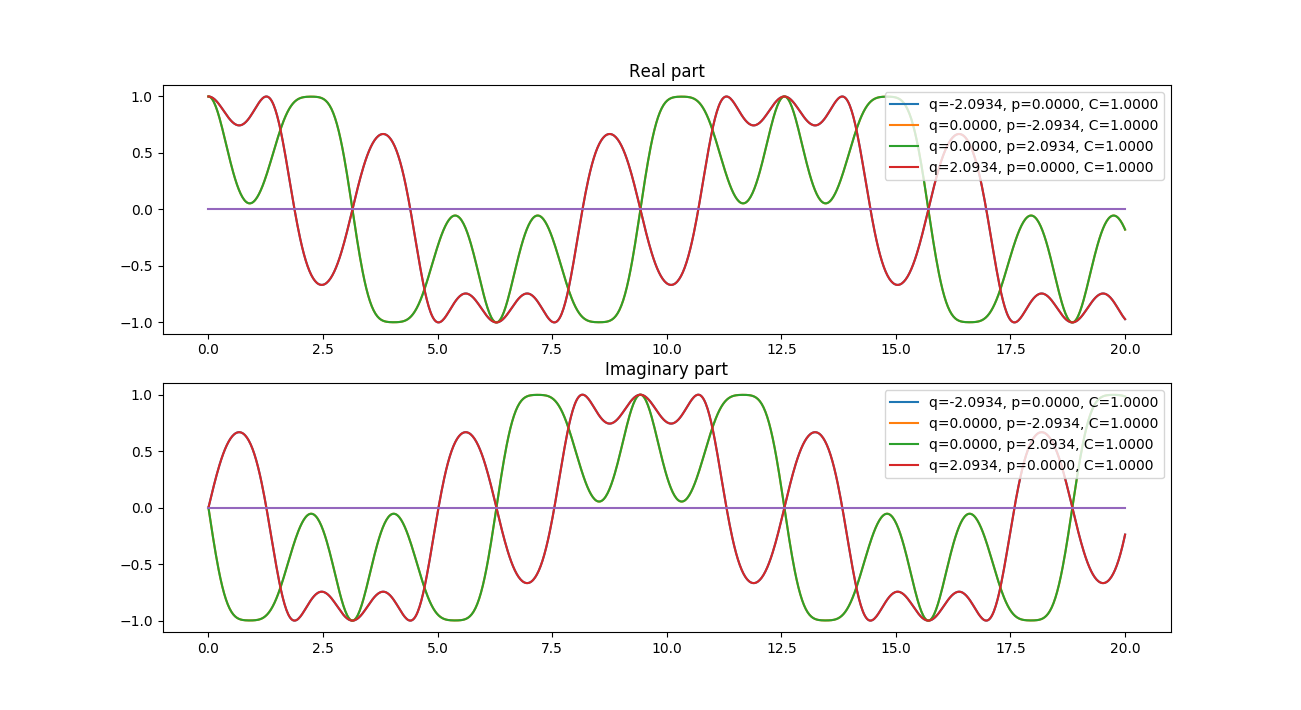
\includegraphics[scale=0.5]{eq_coeff_1.png}
%\caption{Вид коэффициентов (уравнение \ref{eq:coeff}), описываем состояние с энергией $2.5$ с помощью подогнанного базиса, %
%	 можем использовать базисные функции с параметром $\sim$ 0.25 и коэффициентами $[-1.0, 1.0, 1.0, -1.0]$. %
%	 Но такой сигнатуры не получаем. }
%\end{figure}
